\section{问题二：垂荡阻尼参数优化}

\subsection{平均功率目标函数}

仅考虑垂荡时，PTO 输出功率来自阻尼器。线性阻尼的瞬时功率为
\begin{equation}
  P(t)=c(\dot z_b-\dot z_z)^2 .
\end{equation}
非线性阻尼下，阻尼力为 $c|v_r|^\alpha v_r$，其中 $v_r=\dot z_b-\dot z_z$，瞬时功率为
\begin{equation}
  P(t)=c|v_r|^{\alpha+2}.
\end{equation}
为避免初始过渡过程影响参数选择，本文对稳定区间内的功率作时间平均：
\begin{equation}
  \bar P(c,\alpha)=\frac{1}{T_2-T_1}\int_{T_1}^{T_2}P(t)\,dt .
  \label{eq:pavg}
\end{equation}

\subsection{优化方法}

对于线性阻尼，只有 $c$ 一个决策变量，先在 $[1,10^5]$ 上作对数网格粗搜索，再用黄金分割法精修。对于非线性阻尼，同时优化 $c$ 与 $\alpha$，先在 $(\log_{10}c,\alpha)$ 平面上粗扫描判断功率曲面，再采用 Powell 下山法和差分进化进行交叉验证。所有候选解均重新积分并计算稳态平均功率。

\subsection{优化结果}

由当前代码与结果表反推，线性阻尼最优系数为
\[
  c=37420.87\,\mathrm{N\cdot s/m},
\]
对应稳态平均功率约为 $226.60\,\mathrm{W}$。非线性阻尼最优参数为
\[
  c=87064.68,\qquad \alpha=0.3593,
\]
对应稳态平均功率约为 $227.03\,\mathrm{W}$。

\begin{figure}[H]
  \centering
  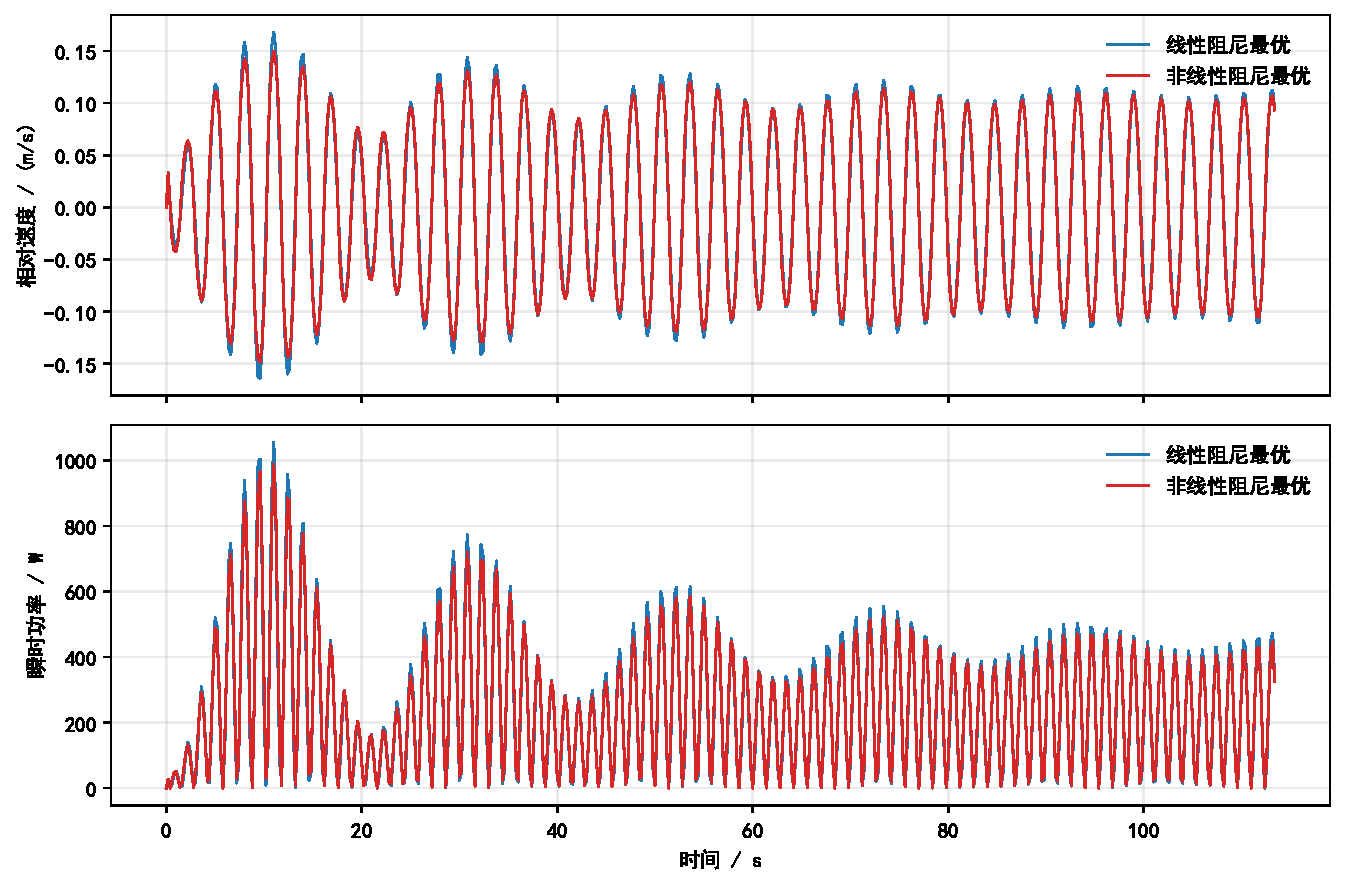
\includegraphics[width=0.90\textwidth]{fig_problem2_power.pdf}
  \caption{问题二最优阻尼参数下的相对速度与瞬时功率}
  \label{fig:p2_power}
\end{figure}

\begin{figure}[H]
  \centering
  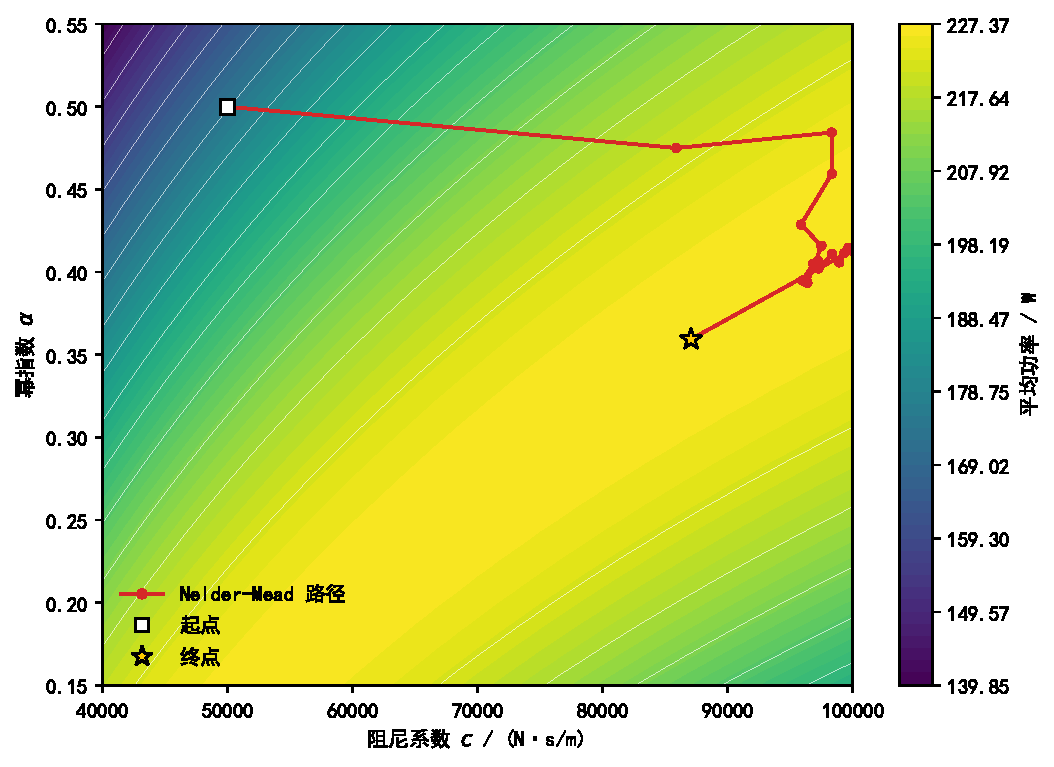
\includegraphics[width=0.58\textwidth]{fig_problem2_avg_power.pdf}
  \caption{问题二两种阻尼模式的稳态平均功率对比}
  \label{fig:p2_avg}
\end{figure}

从图~\ref{fig:p2_avg} 可以看出，非线性阻尼相对于线性阻尼的平均功率提升较小，但其通过幂指数调节不同相对速度区间的阻尼强度，使功率输出略有改善。
